\scanpage{94}

\textcircled{5.} \uline{Classes remarquables d'opérateurs dans l'espace de Hilbert}

Nous commençons par donner un {\color{red}\uline{\color{black}exposé}} de la théorie de Schatten, \deleted{\unsure{qui est|que nous}} sous une forme simplifiée rendue possible par la \deleted{\unsure{lemme}}\inserted{méthode du \unsure{minimum|minimax}} de Weyl, et en {\color{red}\uline{\color{black}y apportant}} q.q \unsure{petits|menus} compléments.

{\reversemarginpar\margin{{\color{red}?}}}

\deleted{\unsure{Déf}} Rappelons la

{\reversemarginpar\margin{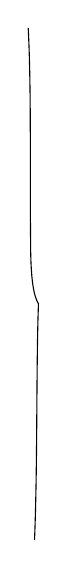
\begin{tikzpicture}[baseline=(current bounding box.north)]\draw[line width=.4pt] (0,0) .. controls (.04,-.8) and (.02,-1.7) .. (.03,-2.7) .. controls (.03,-3.2) and (.07,-3.4) .. (.13,-3.5) .. controls (.10,-4.3) and (.12,-5.5) .. (.08,-6.5);\end{tikzpicture}}}
\uline{Définition 1} \deleted{Soit} Une norme $N$ sur $R^n$ est dite \uline{norme de Schatten} si elle est symétrique, satisfait à

\deleted{\unsure{à|2|3}}

\[
\begin{array}{@{}l@{\qquad}l@{}}
(1)&\displaystyle N(x_1,\mathord{-}x_n)=N(|x_1|,\mathord{-}|x_n|)
\end{array}
\]

\deleted{et si elle} \unsure{si|2.} elle est croissante \deleted{\unsure{sur l'ensem}} sur l'ens. des $x_i\geq 0$, et \deleted{\unsure{est satisf}} est normalisée par $N(1,0,\mathord{-}0)=1$

Une norme $N$ sur $R^{(\underline N)}$ \deleted{$\unsure{R}\underline N$ \unsure{ensemble|espace des}} (\unsure{espace|anneau} des suites infinies \deleted{\unsure{finies}} nulles sauf un nb fini de termes) est appellée une norme de Schatten, si \inserted{pour tout entier $n>0$,} elle induit \deleted{sur} de sur $R^n$ une norme de Schatten

($R^n$ sera ici identifié \deleted{\unsure{à l'espace des suites}}\inserted{au sous-espace} de $R^{(\underline N)}$ formé des suites nulles à partir du rang $n+1$). Notons qu'une norme de Schatten sur $R^n$ induit sur $R^m$ ($m\leq n$) une norme de Schatten. \deleted{\unsure{Tout cette théorie résulte que|Il est immédiat que}}\inserted{Exemples de normes de} Schatten\,:

\deleted{\unsure{Supposons|l'app.}}

\[
\deleted{N_p(\{x_i\})\unsure{=}\left(\sum |x_i|^p\right)^{1/p}\quad\text{\unsure{où }}1\leq p}
\]

les normes $N_p((x_i))=\lVert(x_i)\rVert_p$, définies \unsure{par|pour} \deleted{$1\leq p\leq\unsure{+\infty|\infty}$ \unsure{par}}

{\reversemarginpar\margin{\begin{tikzpicture}[baseline=(current bounding box.north)]\draw[line width=.5pt] (0,0)--(.12,-.22);\end{tikzpicture}}}
\[
\begin{array}{@{}l@{\qquad}l@{}}
(2)&\displaystyle \lVert(x_i)\rVert_p=\left(\sum |x_i|^p\right)^{1/p}\qquad (1\leq p<+\infty)
\end{array}
\]

\[
\begin{array}{@{}l@{\qquad}l@{}}
\deleted{\unsure{4}}\ (3)&\displaystyle \lVert(x_i)\rVert_\infty=\underset{i}{\operatorname{Sup}}\,|x_i|
\end{array}
\]

{\reversemarginpar\margin{\begin{tikzpicture}[baseline=(current bounding box.north)]\draw[line width=.4pt] (-.5,-.12) .. controls (-.6,0) and (-.2,0) .. (0,0) .. controls (.08,-.05) and (.04,-.5) .. (.01,-1.2) .. controls (0,-2.4) and (-.2,-3.4) .. (-.45,-4.2);\end{tikzpicture}}}
Si $N_0$ est une norme de Schatten \deleted{alors} sur $R^n$, il existe toujours une norme de Schatten $N$ sur $R^{(\underline N)}$ \deleted{\unsure{qui}}
{\reversemarginpar\margin{{\color{red}?}}}
{\color{red}\uline{\color{black}induise}} $N_0$\deleted{, \unsure{p. ex.,} \illegible{1}} si, pour \deleted{\unsure{toute|tout}} $x=(x_i)\in\underline{C}_0$, on désigne par
{\reversemarginpar\margin{{\color{red}?}}}
$(\unsure{\rho|R|f}_i(x))$ la suite des $|x_i|$ \deleted{{\color{red}\uline{\color{black}\unsure{rangés|arrangés}}}}\inserted{non nuls}
{\color{red}\uline{\color{black}rangés par ordre de grandeur décro}}issant, on peut p. ex. poser $N(x)=N_0(\rho_1(x),\mathord{-}\rho_n(x))$. Il est trivial

{\reversemarginpar\margin{95}}

